\iflanguage{ngerman}
{\chapter{Methoden und Umsetzung}}
{\chapter{Methods and Implementation}}
\label{sec:methods}


In order to explain the developed proposed solutions, this chapter will first conduct a problem analysis, then a theoretical classification of the explosion views, and finally the implemented methods are explained. 
To illustrate the implementation, first the structure of the program is presented, then the individual approaches are introduced, and finally the VR interaction and surface inspection are demonstrated and the data set and its change over time are discussed.

The problem addressed by this work can be divided into three sub-problems. On the one hand, this is the representation of three-dimensional cells and cell complexes; on the other hand, this is the investigation of possible ways to avoid occlusion and to use immersive techniques and interactions to enable cell and cell surface exploration.
As mentioned in the introductory chapters, different types of explosion views will be tested and compared in order to solve the problem of occlusion.
Special requirements and restrictions apply in this problem scenario, as both the data set and the use of VR technologies necessitate significant changes to traditional explosion views.

Therefore, the \textbf{structure of the data set} should be explained first. %TODO maybe add picture of XML layout? 
It was generated using the Morpheus program and depicts the development of cells over a predetermined time period.
The individual cells consist of voxels which are arranged in a grid layout. Each cell has additional properties such as a unique ID, a cell center and a population to which the cell belongs, as well as data describing the surface properties. 
A population in this context refers to a cell type with unique propagation properties that can be defined in Morpheus.
Different cell populations form a cell complex which is simulated by Morpheus. 
During the simulation, Morpheus then generates snapshots of the current state of the cell complex at regular intervals. 
These are saved as XML files and form the data set used for the visualization in this work. 
In this way, each snapshot describes a temporal state that precisely defines the arrangement of the individual cells in the form of a list of position and surface property values.
The decisive factor here is that the shape and position of an individual cell can change significantly in the course of the simulation. 
The chosen method of occlusion avoidance must therefore take this into account and the visualization should enable the precise inspection of a single cell at any time.

If one now wants to look at the inner cells of the data set and inspect the interaction of the different populations more closely, this is not possible due to the outer cells that cover them. 
So, occlusion occurs because data is obscured by other foreground data.
As demonstrated by Krisanty's example shown in figure \ref{fig:tania}, using cutting planes is not a suitable method of avoiding this problem while still observing the interaction of individual cells with one another.

Explosive views are suitable for viewing the complete data set and, in particular, for looking into the interior of a cell complex and for inspecting individual cells in a targeted manner. 
This type of representation translates the individual parts of a model or dataset in such a way that each part is detached from its touching neighbors.
It should be ensured that the original position of each part is recognizable or comprehensible. 
To achieve this, exploded views should follow the conventions and properties outlined by Li et al. in the background chapter \ref{items:best_practise}.
Exploded views that take these properties into account not only allow for the representation of relative spatial relationships, but also allow the viewer to mentally reconstruct the object being viewed and the arrangement of the individual parts within. 
This is further enhanced when the explosion strength can be adjusted interactively and is therefore a suitable method for the problem at hand.
When drawing or generating an exploded view, the following parameters are of importance and must be specified individually for each exploded object:
\begin{itemize}
	\item \textbf{The canonical axis} of the object, this is the main axis of expansion in which the parts should be exploded to make the mental reconstruction as simple as possible. This depends on many different factors of the object that is being inspected, for mechanical objects this is often related to the assembly order. The definition is more challenging for biological datasets and models. For the dataset at hand, it is not possible to define a clear canonical axis, because the cells change over time and there is no direction in which the propagation of the cells is focused. In this case, it is useful to make the choice of the axis dynamically selectable, as this allows the axis to be adapted to the current state of the cell complex. 
	\item \textbf{The choice of perspective.} Traditional exploded views are often drawn from the side of the object or from slightly above, looking down at the object. An orthographic view is frequently used to better indicate the distance between the individual parts. 
	This is not the case with interactive systems like Li et al.'s, which allow the camera perspective to be adjusted to provide a more realistic representation of the object.\cite{Wilmot_Li_2008}
	Because this work focuses on the use of VR technologies, a perspective view should be chosen. 
	Furthermore, the camera viewpoint is determined by the position of the headset and should change as the user moves. 
	The use of VR headsets allows for a much more intuitive exploration of the data set and aids in understanding the object's composition. 
	One issue with this is that it can cause visual clutter because the user's field of vision may be obscured by scattered parts.
	\item \textbf{View dependent exploded views.} Closely related to the choice of perspective in interactive exploded views is the choice of whether the position of the exploded parts depends on the camera perspective or not. 
	This results in two categories for exploded views in interactive systems.
	View-independent exploded views that transform parts along an axis or away from a point and are not affected by the camera.
	This allows for a more thorough inspection of all parts and the entire model. 
	Each part is displayed in such a way that its position within the whole is discernible.
	View-dependent exploded views are the second type.
	Certain parts or points are chosen here that are always visible regardless of the angle from which they are viewed. 
	This allows for a close examination of specific parts.
	Which of these possibilities is the better one for the given data set has to be investigated.
\end{itemize}

Interactive explosion views can be generated in two different ways. 
Either by calculating the final positions of the exploded parts or by defining forces that push the parts apart to create meaningful explosion views.
Calculating the positions gives more control over the exploded view and allows to display the composition order. 
This is more difficult with force-based systems, since the forces would have to be defined so that no elements overlap and no blocking constraints are violated during the explosion. 
Both methods can generate qualitative exploded views, however, an advantage of the force-based method is that the strength of the forces can easily be adjusted at runtime and thus new explosion views can be generated. 
In this work both methods are implemented and compared, for this the program structure and the utilized tools are briefly explained. 

\section{Implementation}

The dataset is visualized and the exploded views are implemented using Unity 2021.3. %TODO link
Unity is a 3D engine that can be used for game, program and movie development. 
Since it has been developed for over a decade, there are a variety of plugins and resources that can be used to increase development speed. 
It also allows platform-independent development and supports all conventional graphics cards. 
It uses C\# as the programming language for implementing business logic while rendering is implemented natively with C++.  
The Unity-XR-Interaction-Toolkit and the Unity-InputSystem are used for VR support. %TODO link
These are two plugins developed by Unity that simplify the support of all conventional VR headsets by allowing them to be accessed with a unified API.  
The universal rendering pipeline is used for more performant and lightweight rendering. It is a striped down version of unity's standart renderer and allows for more frames per second on mobile devices at the expense of more advanced rendering effects. %TODO link
Since this work is about data visualization and high performance is critical for VR headsets, using this rendering pipeline is beneficial.
An Oculus Quest 2 connected to the computer via Oculus link is utilized to test the implementation. %TODO link

At program start the resource folder is checked for valid Morpheus datasets.
For each existing file that contains a time step, the corresponding Xml-file is read and loaded. 
Since each time step contains information about the cell populations and the states of the individual cells, these are loaded one after the other.
For each time step the program loops through the data set and checks if a cell with the same ID already exists, if this is not the case a new object is created which represents the cell, stores its properties and contains a mesh for each time step of the cell. 
If a cell object with the same ID already exists, a mesh is generated which visualizes the state of the cell and is attached to the cell object as a child object.
At runtime, only the child objects that depict the current time step are active while all others are deactivated.
A manger class allows switching between the different implementations of the exploded views and sends the object transforms that are used to define the exploded positions to the script that drives the explosion. 
An interface implementation of the exploded view method allows for an extendable usage and development. 
A detailed class diagram which clarifies the program structure can be found in the appendix. %TODO create this and link it
For this work, four different methods for generating exploded views were implemented.

%\begin{wrapfigure}{r}{0.59\textwidth}
%	\vspace{-3cm}
%	\hspace{1.5cm}
%	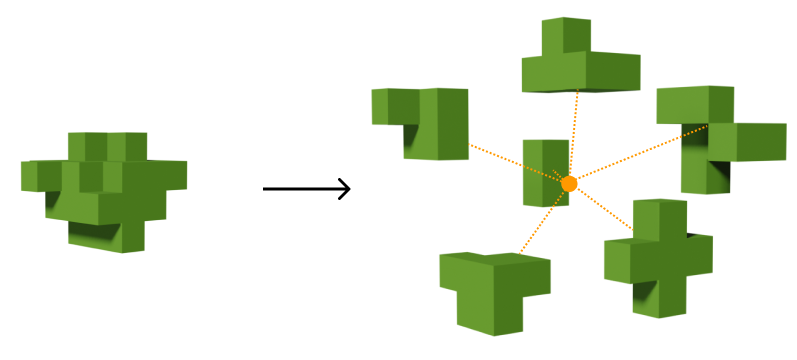
\includegraphics[width=1\linewidth]{fig/Images/PointExplosion}
%	\caption[]{Exploding parts away from a single point}
%	\label{fig:pointExpl1}
%	\hspace{-2.6cm}
%	\vspace{-0.7cm}
%\end{wrapfigure}
\begin{figure}[h]
	\centering
	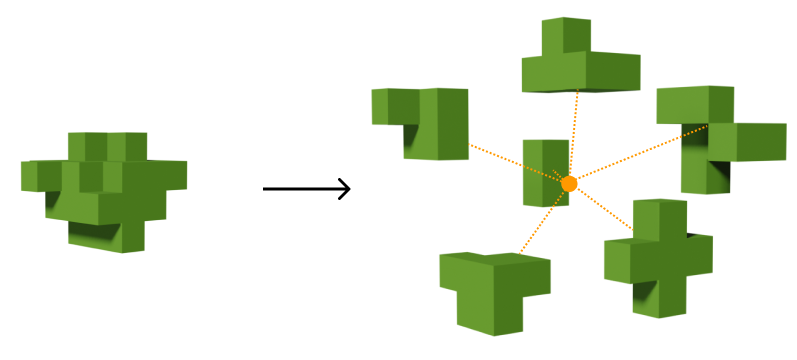
\includegraphics[width=.65\linewidth]{fig/Images/PointExplosion}
	\caption[]{Exploding parts away from a single point.}
	\label{fig:pointExpl1}
\end{figure}

\subsection{Point explosion}
The simplest method to generate an exploded view is to explode from a single point as pictured in figure \ref{fig:pointExpl1}.
The initial position of the cells, which is read from the data set, is used as a reference point $P_o$. 
The user can then place a control point $P_c$ at any position from which the explosion originates. 
The new position of the parts is thus determined by the translation along the linear line, which is defined by the control point and the initial reference point.
The target position $P_t$ is determined for each part $P_i$ by the following formula. 
\begin{equation}
	P_t = P_o + (P_o - P_c) * F_{max}
	\label{eq:pointExpl1}
\end{equation}
Here, $F_{max}$ is a constant factor that describes the maximum explosion distance. At the end the position of the part is determined by interpolating between the reference point $P_o$ and the target point $P_t$ with the user adjustable explosion strength $F_e \in [0, 1]$.
It must be ensured that the points are in the same coordinate system, this is not always the case with my implementation, since the individual parts are child objects of a container object, which allows the data set to be scaled.
To clarify the spatial relations, a further adjustable factor $F_l$ has been added which is scaled with the length of the vector from the control point $P_c$ to the initial position $P_o$. This can be used to amplify the spatial distances and to restrict the view to nearby objects.
The final target position is thus described by the following formula:
\begin{equation}
	\vec{d} = (P_o - P_c) 
	\label{eq:pointExpl2}
\end{equation}
\begin{equation} 
	P_t = P_o + \hat{d} * F_{max} + \vec{d} * F_l * \|d\|
	\label{eq:pointExpl3}
\end{equation}
The point explosion is particularly suitable for selecting parts in a targeted manner and for examining them more closely.
This is a view independent explosion view, because the position of the camera has no effect on the position of the parts. 
However, this method does not take into account any blocking directions and relations. 
Enclosed objects are also not recognized and could remain hidden.
Furthermore, there is no consideration of the canonical axes of an object.
The method is similar to the implementation of the explosion probe by Sonnet et al.\cite{Sonnet_2004} but has no effect radius, so all parts, no matter how far away from the control point, are pushed away.

\subsection{Line explosion} 
%\begin{wrapfigure}{r}{0.59\textwidth}
%	\vspace{-3cm}
%	\hspace{1.5cm}
%	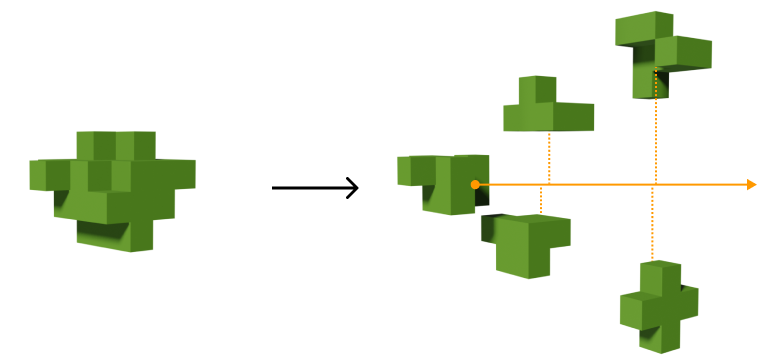
\includegraphics[width=1\linewidth]{fig/Images/LineExplosion}
%	\caption[]{Exploding parts away from an axis defined by two points. The control point $P_s$ is marked as a yellow dot on the left side of the line, point $P_d$ as an arrow.}
%	\label{fig:lineExpl1}
%	\vspace{-0.7cm}
%	\hspace{-0.6cm}
%\end{wrapfigure}
\begin{figure}[h]
	\centering
	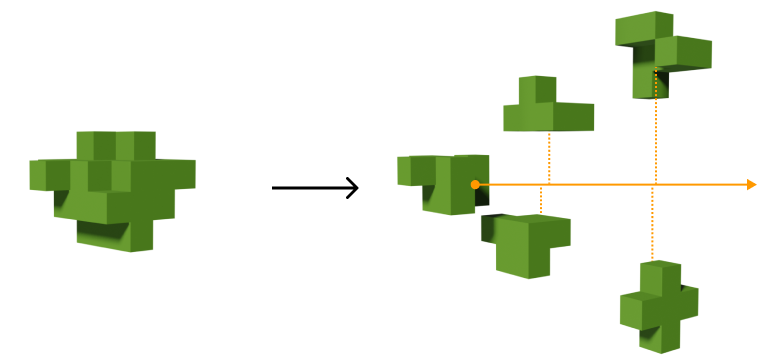
\includegraphics[width=.65\linewidth]{fig/Images/LineExplosion}
	\caption[]{Exploding parts away from an axis defined by two points. The control point $P_s$ is marked as a yellow dot on the left side of the line, point $P_d$ as an arrow.}
	\label{fig:lineExpl1}
\end{figure}

An expanded exploded view that allows more control is achieved by defining a line and transforming the parts away from that line, as shown in figure \ref{fig:lineExpl1}.
This is achieved by allowing the user to set two control points in space, a line is then drawn between these two control points. 
The first of the control points $P_s$ indicates the starting position of the line, the second point $P_d$ the direction in which the line should progress. 
Now each part is projected onto this axis, if this projection lies in front of the starting point, the part is pushed away from this projection point. 
By moving the control points, it is possible to select which parts of the model will explode from their original position and which will remain rigid. 
Moving the control point that defines the direction of the axis allows the user to create different explosion views.
The projection $P_{proj_i}$ of each part $P_i$ onto the defined line can be calculated by projecting the vector $\vec{d_p}$ that goes from the starting point $P_s$ to the respective part onto the line $\vec{d_{ab}}$ that passes through the two control points. 
The projection point is thus given by the following formula:
\begin{equation}
	P_{proj_i} = P_s + \frac{\langle\vec{d_p},\vec{d_{ab}}\rangle}{\langle\vec{d_{ab}},\vec{d_{ab}}\rangle} * \vec{d_{ab}}
	\label{eq:LineProj}
\end{equation}
The target position sought can then be determined by multiplying the vector $\vec{d_{expl}}$, which runs from the calculated point $P_{proj_i}$ to the reference position of the part, by the explosion strength $F_e$.
In order to enable a targeted determination of the effected parts, only those parts are exploded where the dot product of the vectors $\vec{d_{aProj}}$, which is defined by the starting point of the line $P_s$ and the point $P_{proj_i}$, and the line $\vec{d_{ab}}$ is equal to one.
This allows the user, for example, to explode only half of the parts of the object and leave the remaining parts in their original position to get a better understanding of the object. 
To improve the display and make it suitable for each type of cell, three further customizable factors have been introduced that change the target position of the parts and thus generate different explosion views. 
This makes it possible to customize the shape of the exploded view.
\begin{itemize}
	\item The first factor $F_1$ amplifies the distance between the starting point $P_s$ of the line and the projection point $P_{proj_j}$ of the part. 
	This allows to adjust the length of the body of the exploded view and to clarify the distances between the individual parts.  
	\item The second factor $F_2$ amplifies the strength of explosion of the part based on the distance of the part's projection point to the starting point $P_s$ of the line. 
	This causes a cone shape of the explosive body, i.e. the area where the parts explode.
	\item The third factor $F_3$ adds a constant value to the explosion vector $\vec{d_{expl}}$. 
	This leads to a cylindrical explosion view or can be used to enlarge the explosion in case of a low explosion strength.  
\end{itemize}
By adjusting these three factors, different explosion views can be generated. The different possibilities with the corresponding factors can be seen in Figure \ref{fig:LineExplosionFactors}.
The explosion can be thought of as a cone or a cylinder, whose shape can be adjusted using the parameters $F_1$ to $F_3$.
The factor $F_1$ increases the distance between the parts along the defined line, which ideally is placed on the canonical axis of the model. This increases the distance between the parts, which can be thought of as increasing the height of the cylinder.
The radius of the side of the explosion cylinder that is further away from the starting point can be changed with the factor $F_2$. Thus, the expansion of the parts further away from the control point $P_s$ can be increased and a cone-shaped exploded view can be created. 
The factor $F_3$, on the other hand, adjusts the radius of the base of the cylinder. %TODO add possible exploded view that can be createt or put this in results
\begin{figure}[h]
	\centering
	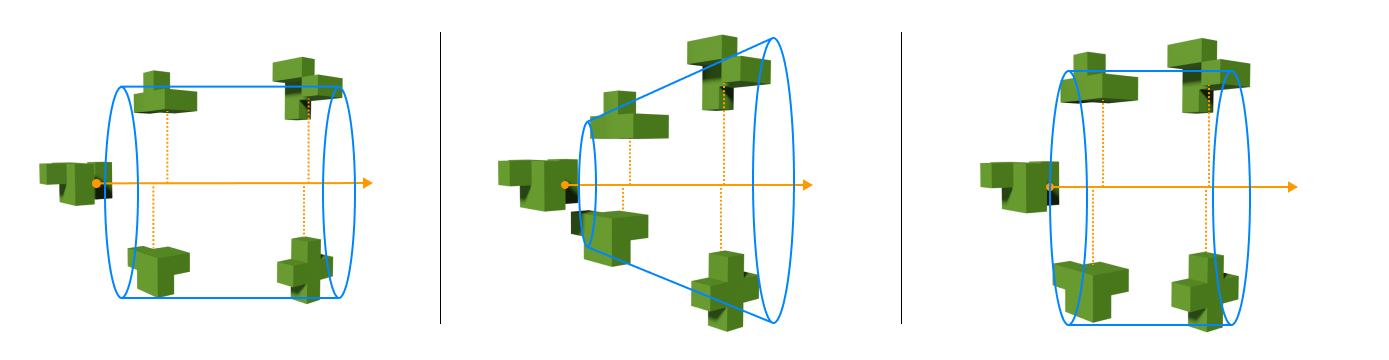
\includegraphics[width=.9\linewidth]{fig/Images/LineExplosionFactors}
	\caption[]{Influence of the factors $F_1$ (left), $F_2$ (middle) and $F_3$ (right) on the shape of the exploded view.}
	\label{fig:LineExplosionFactors}
\end{figure}
The final calculation of the target point is shown in Figure \ref{fig:LineexplosionCode}.
Again, it must be ensured that all points and directions are in the same coordinate system; this was not taken into account in Figure \ref{fig:LineexplosionCode}. The complete implementation can be found on the GitHub page. %TODO cite github
The line explosion diagram calculated by this method is also view-independent, since the camera has no influence on the target position of the parts.  
It is also possible to place the line in the canonical axis of the object and thus expand it.  
\begin{figure}[ht]
	\begin{lstlisting}
List parts
Position a, b
Float F1, F2, F3

function Explode(float F_e){
	var AB = b - a
	
	foreach(part in parts){
		var d_p = part.position - a
		var proj = a + DotProduct(d_p, AB) / DotProduct(AB, AB) * AB
		
		var d_expl = part.position - proj
		var d_a_proj = proj - a
		
		if(DotProduct(AB, proj) == 1){
			part.targetPosition = part.initalPosition + d_expl.normalized * F3
			+ d_a_proj.magnitude * F1 * d_expl.normalized
			+ d_a_proj * F2
		}
		else
		part.targetPosition = part.initalPosition
		
		//LinearInterpolate(a, b, c) is a function that linearly interpolates from Position a to a Position b, by c
		//so the returned value is a + (b - a) * c
		part.position = LinearInterpolate(part.initialPosition, part.targetPosition, F_e)
	}
}
	\end{lstlisting}
	\caption{This shows a pseudo code implementation of the algorithm used for exploding the parts away from a line.}
	\label{fig:LineexplosionCode}
\end{figure}
\subsection{Head-mounted line explosion}
This method is based on the same implementation as the line explosion, but extended to make it view dependent. 
The only difference is that the control point $P_d$ which determines the direction of the line is set to be the same as the position of the headset in that frame. 
When the first control point is set within the object, an exploded view is created, allowing the user to look into the object dynamically. 
All parts that are in front of the first control point are automatically moved away. 
This technique allows the user to walk around the object to inspect the interior of the cell from any angle.
A function has also been added that stops updating the position of the point $P_d$, turning the function into the previously described line explosion and allowing the user to examine specific parts. 

\begin{figure}[h]
	\centering
	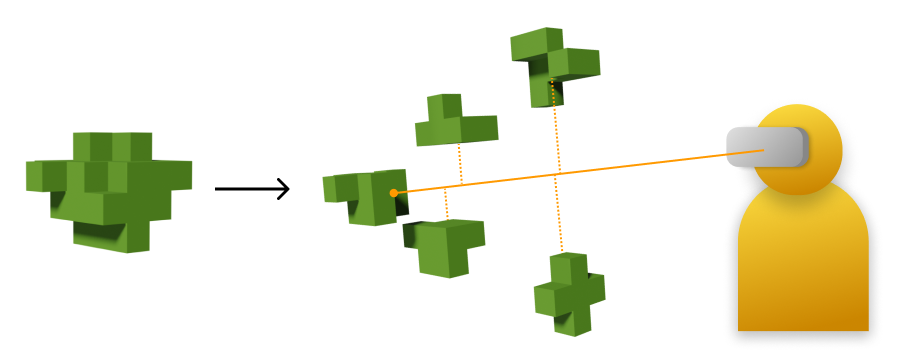
\includegraphics[width=.65\linewidth]{fig/Images/LineExplosionHeadMounted}
	\caption[]{Concept of the head-mounted explosion. The point $P_d$ is set to be the same as the headsets position. This allows a clear view onto the leftmost part, no matter from which angle the user looks. }
	\label{fig:headExpl}
\end{figure}

\subsection{Force-based explosion}
Unlike the previous techniques, this method determines the exploded position of the parts using a force-based approach.
This approach is based on the same principles described by Bruckner et al., but the forces described by Bruckner et al. have been adapted to give good results with the existing program structure.\cite{Bruckner_2006}
In comparison to Bruckner et al.'s method, however, the reference points of the parts are used to apply the forces and not the vertices of a volumetric data set.
To create an explosion view, the user selects the desired target parts. 
It is possible to select multiple target parts, these are only affected by the return force and remain in their original position.
Now four forces with different strengths are applied to all parts which push them away and allow a free line of sight to the selected parts.
The four forces acting on each part are defined as follows:
\begin{itemize}
	\item The first force is the \textbf{return force}, which causes the pieces to be pushed back to their original position.
	The first force is the return force, which causes the parts to be pushed back to their original position. 
	For this, the vector $r$ which goes from the current position of the part to its original position is calculated and the part is pushed in the direction of this vector. 
	To reduce the jittering when the parts are close to their original point, the vector $r$ is normalized and multiplied by the logarithm of its length. 
	This reduces the strength of the force when the length of the vector is small. 
	The following formula is therefore used to describe the force. 
	It is identical to the formula used by Bruckner et al. and affects every part.
	\begin{equation}
		F_r = c_r * ln(\|r\|) * \hat{r}
		\label{eq:FB_return}
	\end{equation}
	Here, the constant term $c_r$ refers to a variable that affects the force's strength.
	
	\item Any piece that is not a selected target piece is affected by the \textbf{explosive force} $F_e$. This pushes all parts apart and creates the exploded view, it emanates from each target part. 
	It can be described by the following formula:
	\begin{equation}
		F_e = \frac{c_e}{e^{\|r\|}} * \frac{c_e}{P_{count}} * r * f_{expl}
		\label{eq:FB_explosion}
	\end{equation}
	Where $c_e$ is again a constant factor, $r$ is a vector that goes from the target part to the part being handled and $f_expl$ is a factor that amplifies the force. 
	$c_e$ is a value between zero and one that can be determined by the user, which is why the factor $f_{expl}$ was introduced to amplify the force. 
	The strength of the force is divided by the number of target parts $P_{count}$ to remain constant. 
	
	\item The \textbf{viewing force} $F_v$ makes the explosion diagram view-dependent. 
	This is achieved by calculating an axis from the headset to each selected target part, from which other, non-target, parts are pushed away. 
	The projection of each part onto the axis is calculated using the same formula \ref{eq:LineProj} introduced earlier in Line Explosion.
	The direction $r$ in which the parts are pushed is thus determined from the projection point of the equation and the position of the part. 
	The strength of the force is then calculated as follows and applied to each part that is not a target part:
	\begin{equation}
		F_v = \frac{c_v}{\|r\|} * \hat{r}
		\label{eq:FB_viewingForce}
	\end{equation}
	The strength of the force $F_v$ is here divided by the length of the vector $r$, this is useful to minimize the distance of the pushed away parts from their original position. 
	Here, each part is pushed away no matter whether the projection of the considered part is behind or in front of the currently considered target part. 
	This results in less visual clutter, since the target part is clearly separated from other parts and can be seen directly on the background without other parts behind it crowding the view. 
	$c_v$ is again a constant factor which allows the strength of the force to be adjusted.
	\item The \textbf{spacing force} $F_s$ is responsible for preventing the pieces from overlapping and acts from any piece that is not a target piece to any other non-target piece. It is calculated as follows:
	\begin{equation}
	F_s = \frac{c_s}{\|r\|^2} * \frac{r}{P_{count}}
	\label{eq:FB_spacingForce}
	\end{equation}
	Here $c_s$ is again a constant force, which is variable and adjusts the strength of the force. 
	The vector $r$ runs from the currently treated part $P_i$ to the other part $P_j$, while $P_{count}$ is the total count of all parts. 
	This is used to normalize the force. 
\end{itemize}
The individual forces can thus be adjusted by the variables $c_r$, $c_e$, $c_v$ and $c_s$ to generate different resulting representations. 
An advantage compared to the other methods is that it is possible to select any number of target parts. Since they remain at their original position, they can be viewed in detail and their environment can be observed.   
Unity's physics engine is used to dampen the movement of the parts over time, preventing possible jittering of the parts. 
However, this can also lead to a delay when changing the position of the parts, which reduces the responsiveness of the motion.
For all methods there is the possibility to visualize the most important directions used for the calculations by lines. 
This is to facilitate the comprehension of the applied methods and to make it easier for the user to understand the transformation of the parts.

\subsection{VR interaction}

All non-force based techniques presented are operated by control points that can be placed in the scene using a ray interactor. 
This allows the user to point to the control points and dynamically adjust their position. %TODO add picture of controlpoints
Furthermore, a user interface was implemented that allows the user to adjust all important parameters of the individual methods. 
So the best representation can be found at runtime.  
Additionally, a UI panel that enables the control of the time steps and subsequently permits the selection of a particular time step was added.
At any time, it is possible for the user to separate out individual parts and take a closer inspection. 
The part is then placed in front of the user and can be rotated and scaled with the control keys. Furthermore, a UI panel shows the ID and population to which the cell belongs. 
Grabbing a cell therefore enables basic surface inspection but the displayed information is limited and could be improved and expanded in future work. 

\subsection{dynamic data sets for exploded views}

A major problem that arises in the visualization is the temporal change of the data set. This is to be solved in two different ways.
On the one hand, the change in the cell over time is visualized and displayed with less opacity.
It can be selected how many previous time steps are displayed at the same time.
This allows to view the temporal change of the cell over a period of time. %TODO add pictures 
The second approach adjusts the reference point used to determine the exploded position. 
This is set, at the user's request, from the centers of mass defined in the data set and interpolated between the individual time steps.
The reference position of the last time step is defined as the starting point, now it is interpolated to the reference position of the current time step. This happens over the time with which the time steps are changed. 
A problem that can occur is that the parts are close to the projection lines that are calculated to determine the target position. 
If this is the case, the target position can change abruptly, when the used reference point jumps over the projection line and cause a lot of visual movement which makes the inspection of individual areas difficult.  
In the dataset used for testing, it was found to be more useful to use the initial position of the cell as a permanent reference point. 
However, this has the obvious disadvantage that the cell can move far away from this initial point over the simulation, which can complicate the spatial comprehension of the structure. 



